\documentclass{article}
%\usepackage[brazil]{babel}
\usepackage[utf8]{inputenc}
\usepackage{geometry}
\usepackage{tikz}
\usepackage{amsmath}
\usepackage{amssymb}
\usepackage{graphicx,xcolor,lipsum,multicol,caption}
\usetikzlibrary{arrows.meta,
	chains,
	fit,
	positioning,
	quotes}
\usepackage{pdfpages}


\begin{document}
		\begin{titlepage}
		\begin{center}
			{\large \textbf{Universidade Federal do Rio de Janeiro}}

			\vspace{9cm}	
			
			{\Large \textbf{Biostar Catalogue}}\\
			
			\vspace{9cm}
			
			\textbf{Rio de Janeiro, maio de 2024}
		\end{center}	
	\end{titlepage}
	
	\newpage
	\begin{center}
		\section*{\small Catálogos}
	\end{center}
	\vspace{50pt}	
	
	
	\begin{figure}[h]
		\centering
		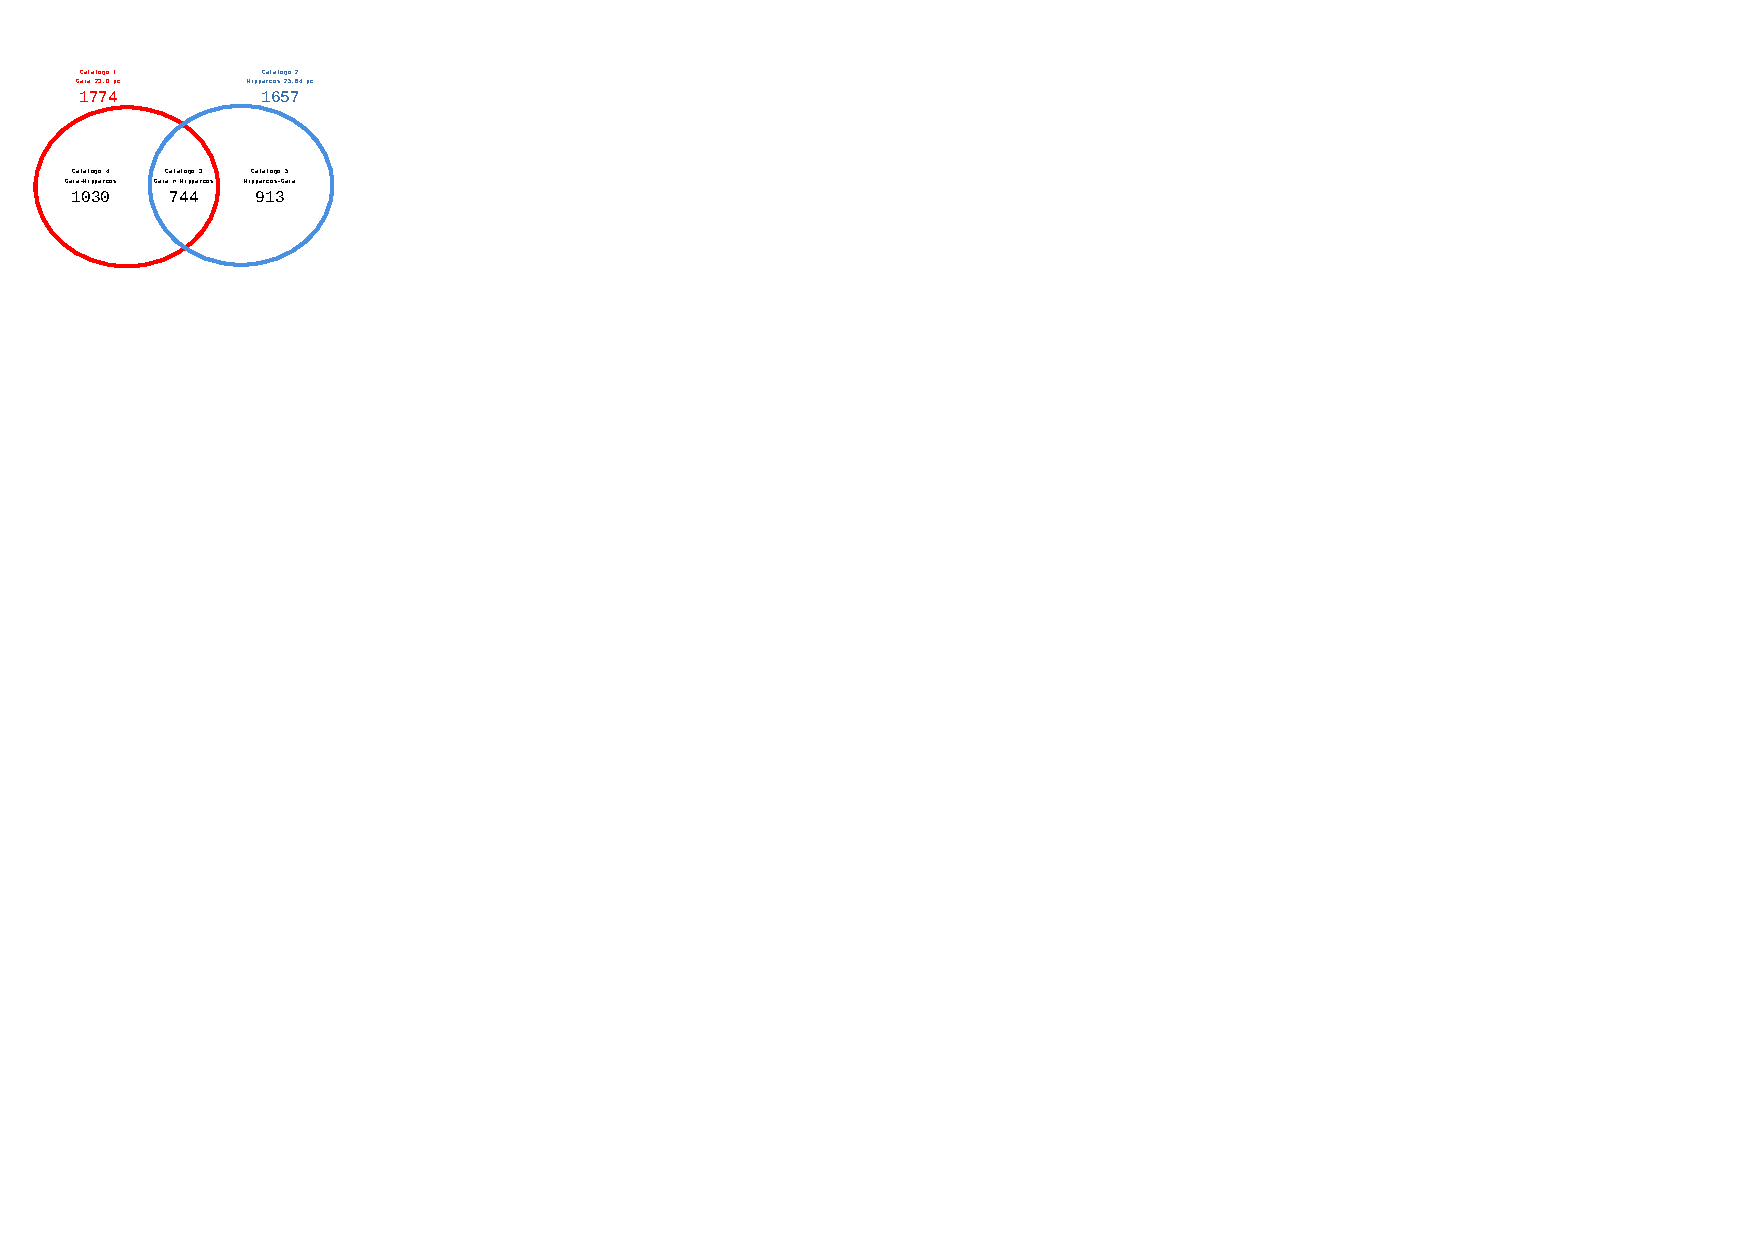
\includegraphics[width=\textwidth, trim = 0cm 16.4cm 23cm 1.1cm, clip]{catalogues.pdf}
		%trim=left bottom right top
		\caption*{\scriptsize diagrama de Venn dos catálogos}
	\end{figure}
	
	\newpage
	\begin{center}
	\section*{\small Fluxograma do Algoritmo de Interseção}
	\end{center}
	\vspace{50pt}	
	
	
	\begin{figure}[h]
		\centering
		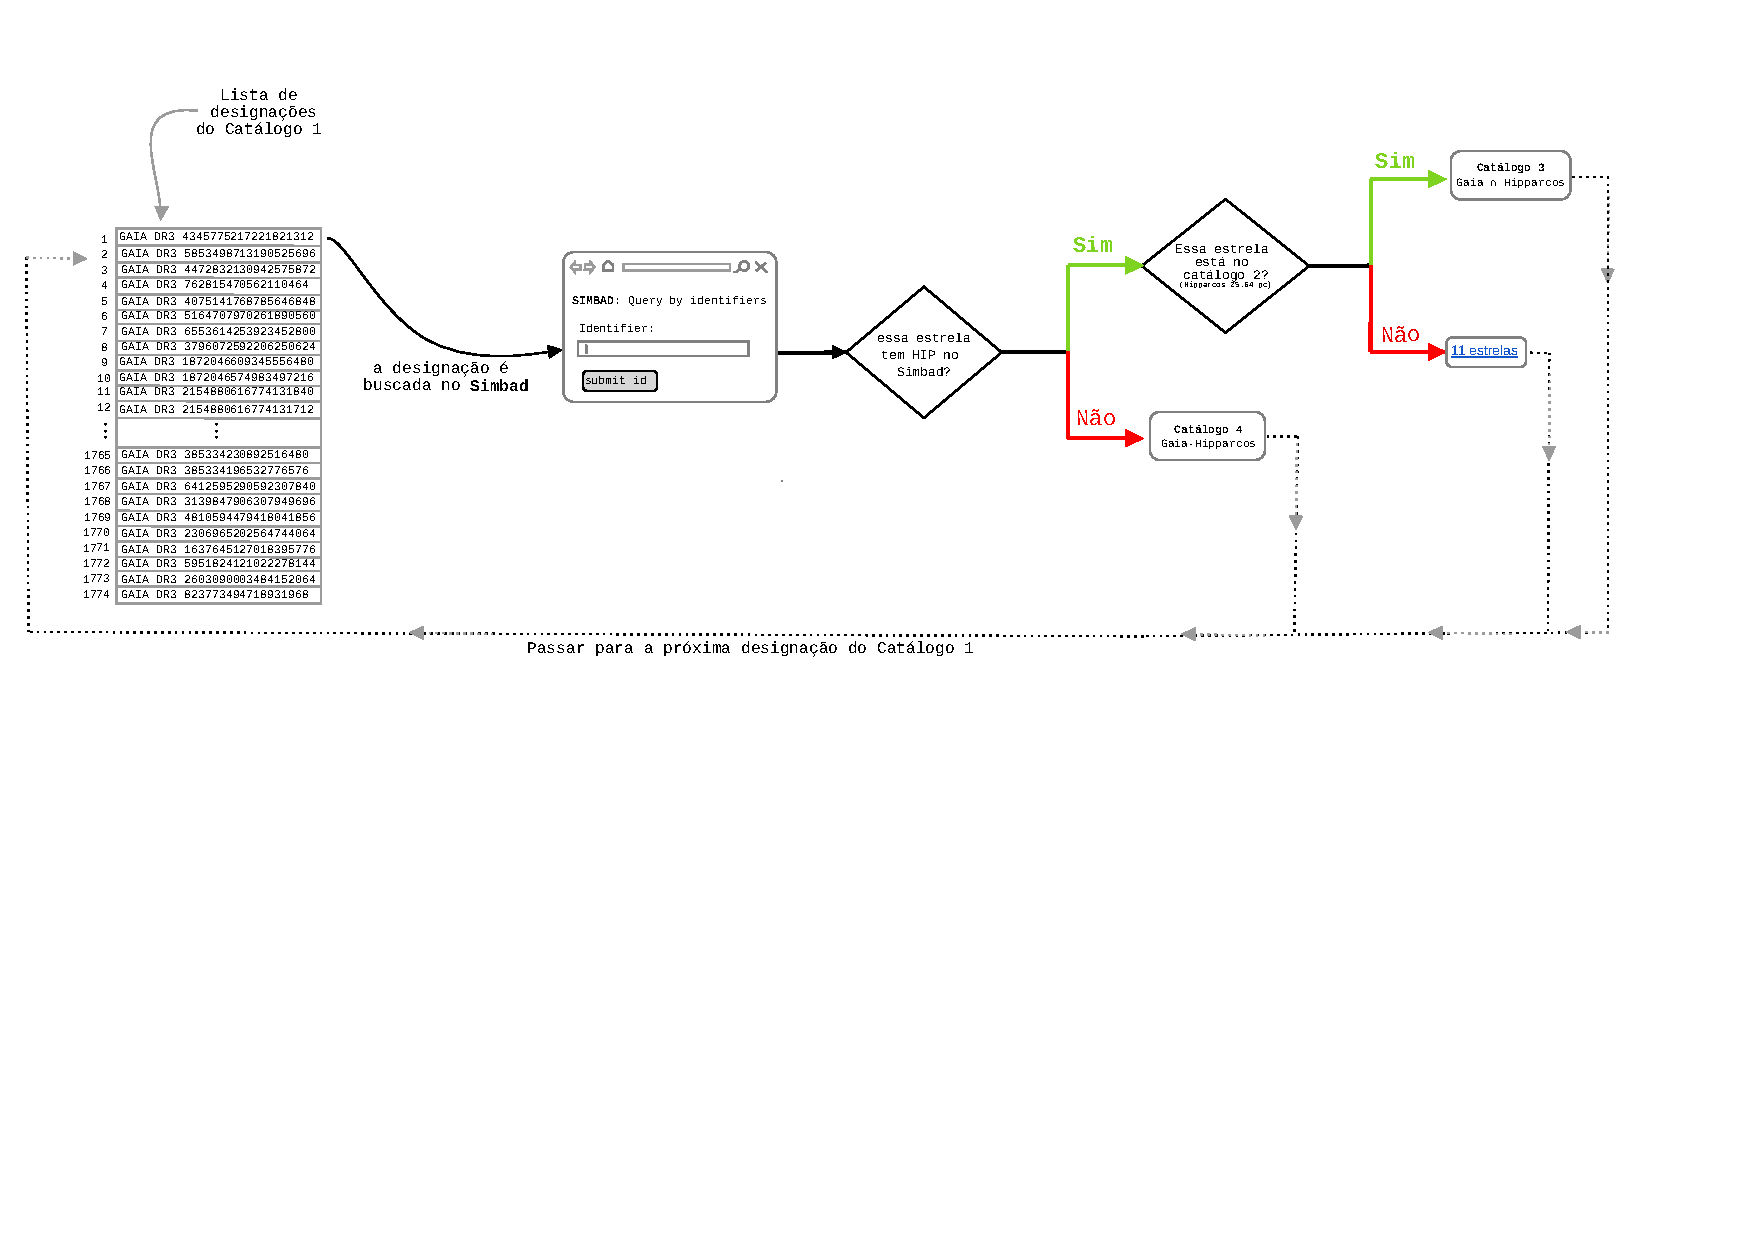
\includegraphics[width=\textwidth, trim = 0cm 9cm 0cm 1cm, clip]{diagramintersection.pdf}
		%trim=left bottom right top
		\caption*{\scriptsize fluxograma do algoritmo de interseção (Gaia $\cap$ Hipparcos)}
	\end{figure}

	\newpage
	\begin{center}
		\section*{\small Exemplo de resultado do algoritmo da página anterior}
	\end{center}
	\vspace{50pt}	
	
	
	\begin{figure}[h]
		\centering
		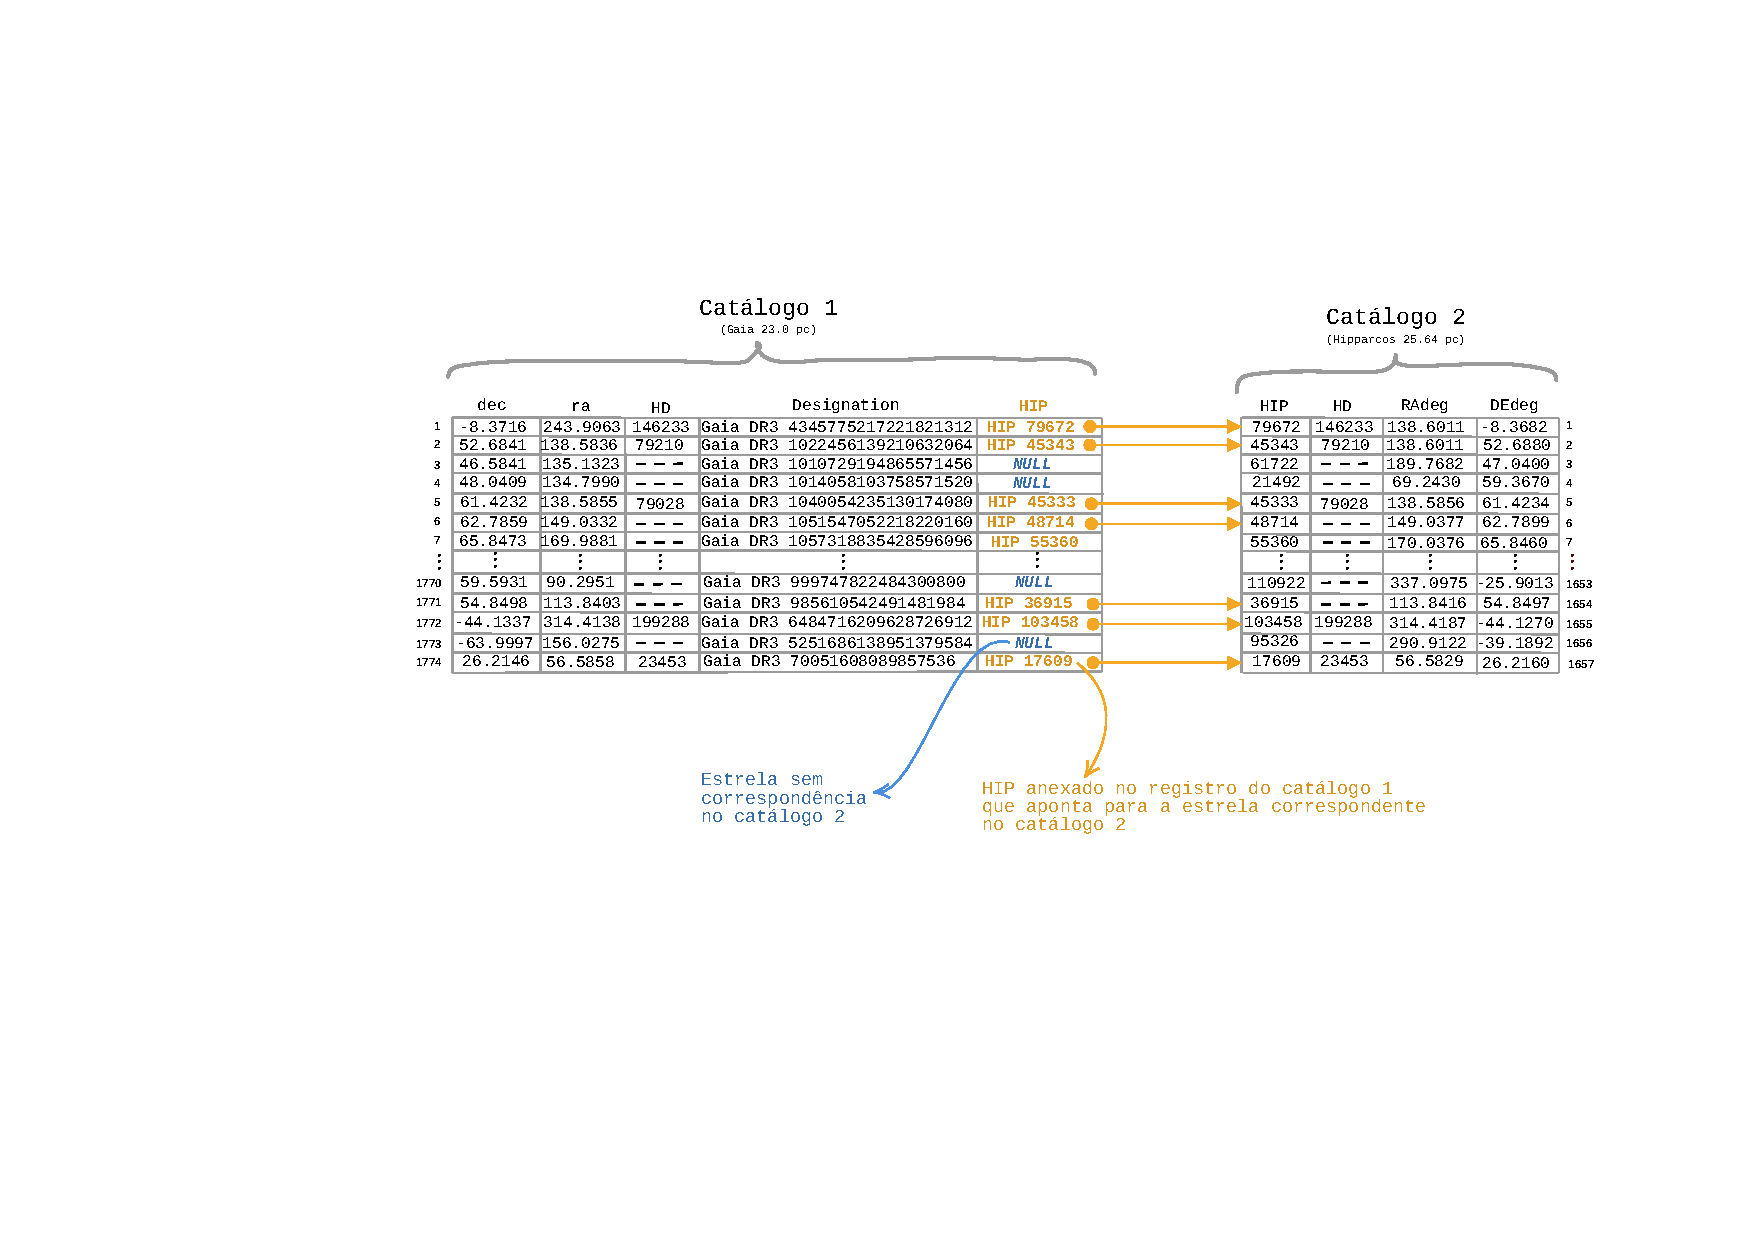
\includegraphics[width=\textwidth, trim = 7cm 6.8cm 2.7cm 5cm, clip]{exemplificando.pdf}
		%trim=left bottom right top
		\caption*{\scriptsize exemplificando o resultado do algoritmo da página anterior}
	\end{figure}
	
	%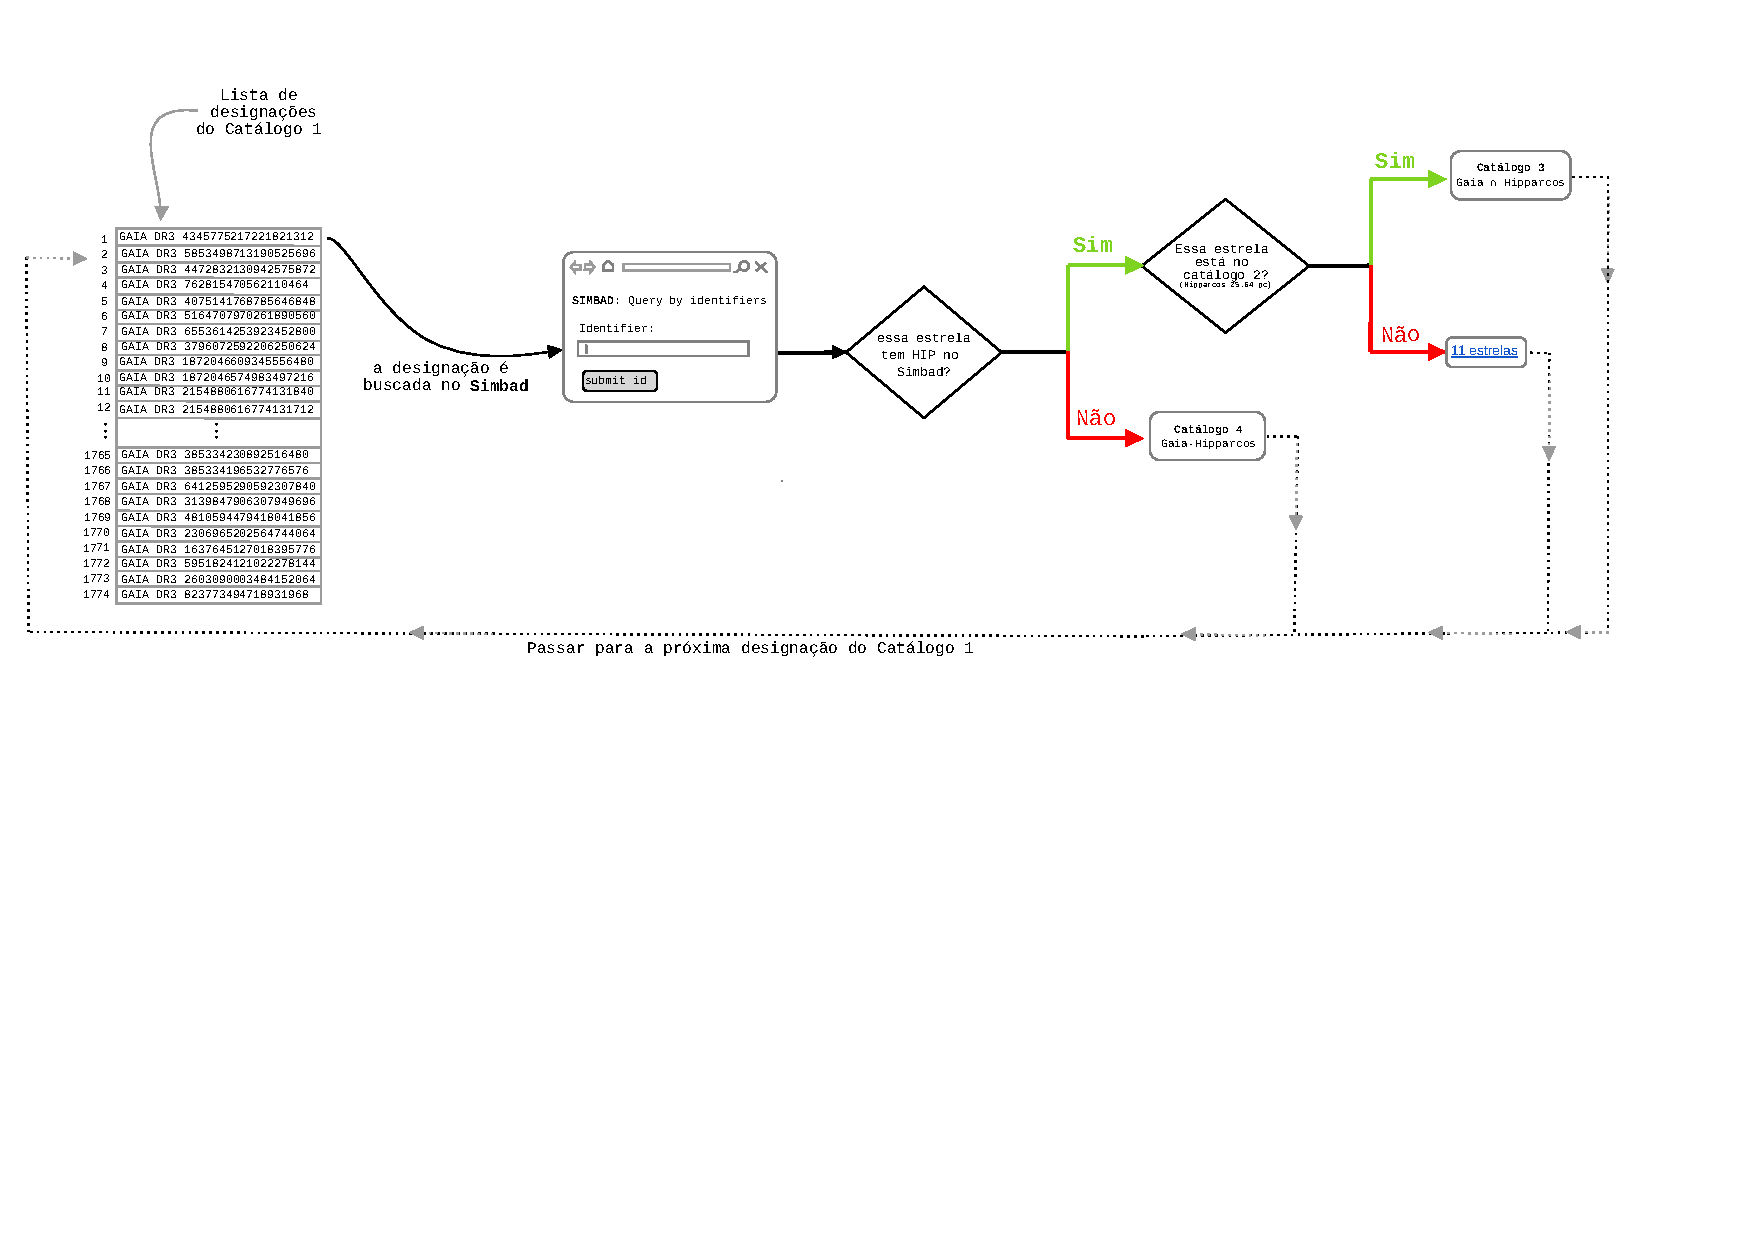
\includepdf[pages={1}]{diagramintersection.pdf}
	
\end{document}